\documentclass[a4paper]{book}
\usepackage{makeidx}
\usepackage{natbib}
\usepackage{graphicx}
\usepackage{multicol}
\usepackage{float}
\usepackage{listings}
\usepackage{color}
\usepackage{ifthen}
\usepackage[table]{xcolor}
\usepackage{textcomp}
\usepackage{alltt}
\usepackage[utf8]{inputenc}
\usepackage[T2A]{fontenc}
\usepackage[russian]{babel}

\usepackage{mathptmx}
\usepackage[scaled=.90]{helvet}
\usepackage{courier}
\usepackage{sectsty}
\usepackage[titles]{tocloft}
\usepackage{doxygen}
\lstset{language=C++,inputencoding=utf8,basicstyle=\footnotesize,breaklines=true,breakatwhitespace=true,tabsize=8,numbers=left }
\makeindex
\setcounter{tocdepth}{3}
\renewcommand{\footrulewidth}{0.4pt}
\renewcommand{\familydefault}{\sfdefault}
\hfuzz=15pt
\setlength{\emergencystretch}{15pt}
\hbadness=750
\tolerance=750
\begin{document}
\begin{titlepage}
\vspace*{7cm}
\begin{center}
{\Large \-Table \-Driven \-Parser }\\
\vspace*{1cm}
{\large Создано системой Doxygen 1.7.6.1}\\
\vspace*{0.5cm}
{\small Ср 1 Фев 2012 08:16:03}\\
\end{center}
\end{titlepage}
\clearemptydoublepage
\pagenumbering{roman}
\tableofcontents
\clearemptydoublepage
\pagenumbering{arabic}
\chapter{Алфавитный указатель классов}
\section{Иерархия классов}
Иерархия классов.\begin{DoxyCompactList}
\item \contentsline{section}{\-Grammar\-Symbol}{\pageref{classGrammarSymbol}}{}
\item \contentsline{section}{\-Lexer}{\pageref{classLexer}}{}
\begin{DoxyCompactList}
\item \contentsline{section}{\-Code\-Lexer}{\pageref{classCodeLexer}}{}
\item \contentsline{section}{\-Grammar\-Lexer}{\pageref{classGrammarLexer}}{}
\end{DoxyCompactList}
\item \contentsline{section}{\-Surround\-Chars}{\pageref{structSurroundChars}}{}
\item \contentsline{section}{\-Table\-Driven\-Parser}{\pageref{classTableDrivenParser}}{}
\item \contentsline{section}{\-Token}{\pageref{structToken}}{}
\end{DoxyCompactList}

\chapter{Алфавитный указатель классов}
\section{Классы}
Классы с их кратким описанием.\begin{DoxyCompactList}
\item\contentsline{section}{{\bf \-Code\-Lexer} \\*Лексический анализатор для программного кода }{\pageref{classCodeLexer}}{}
\item\contentsline{section}{{\bf \-Grammar\-Lexer} \\*Лексический анализатор для работы с описанием КС-\/грамматики }{\pageref{classGrammarLexer}}{}
\item\contentsline{section}{{\bf \-Grammar\-Symbol} \\*Описывает символ грамматики }{\pageref{classGrammarSymbol}}{}
\item\contentsline{section}{{\bf \-Lexer} \\*Лексический анализатор }{\pageref{classLexer}}{}
\item\contentsline{section}{{\bf \-Surround\-Chars} \\*Описание символов, окружающих лексему }{\pageref{structSurroundChars}}{}
\item\contentsline{section}{{\bf \-Table\-Driven\-Parser} \\*Синтаксический нерекурсивный предиктивный анализатор \-L\-L(1)-\/грамматик }{\pageref{classTableDrivenParser}}{}
\item\contentsline{section}{{\bf \-Token} \\*Токен полученный из лексемы входного потока }{\pageref{structToken}}{}
\end{DoxyCompactList}

\chapter{Классы}
\section{Класс \-Code\-Lexer}
\label{classCodeLexer}\index{\-Code\-Lexer@{\-Code\-Lexer}}


Лексический анализатор для программного кода  




{\ttfamily \#include $<$\-Code\-Lexer.\-h$>$}

Граф наследования\-:\-Code\-Lexer\-:\begin{figure}[H]
\begin{center}
\leavevmode
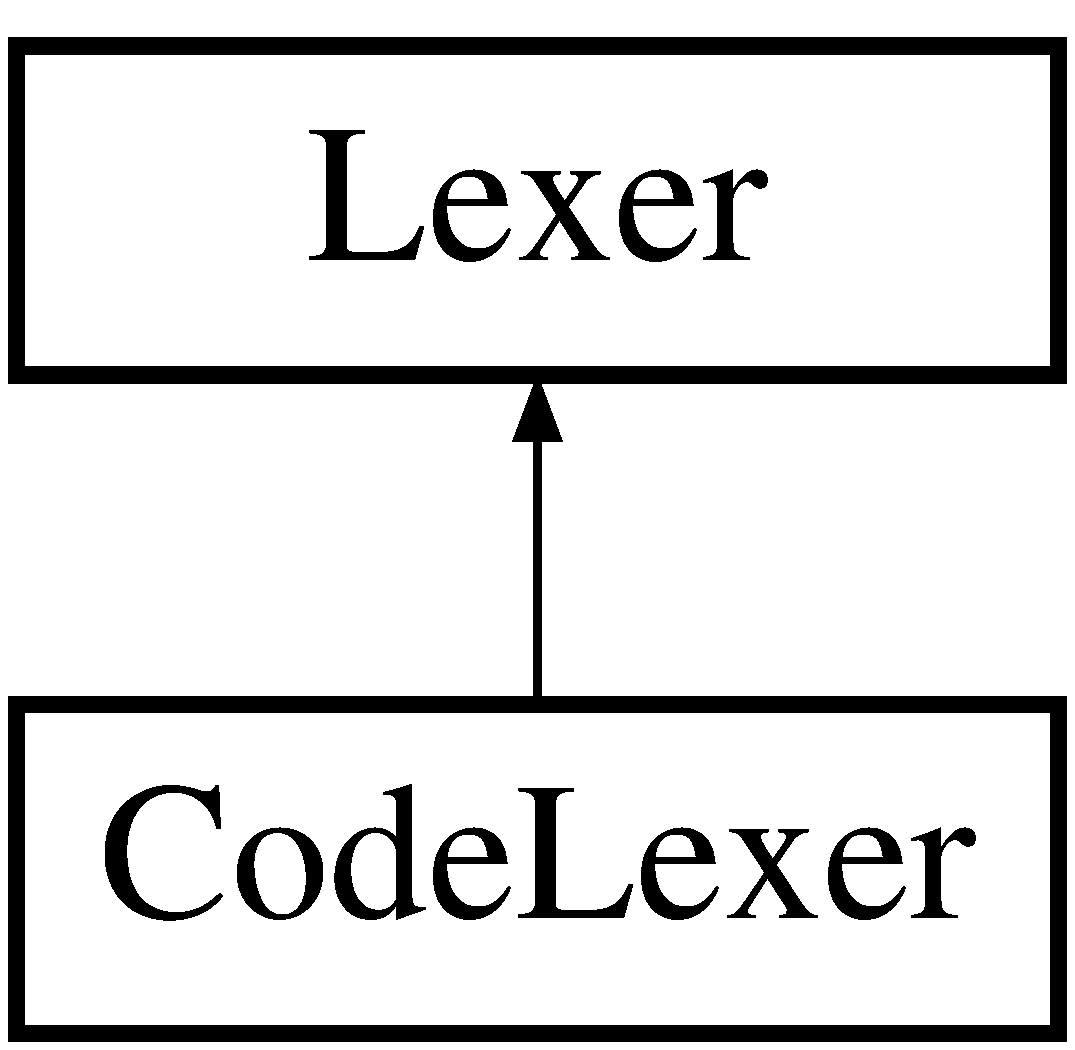
\includegraphics[height=2.000000cm]{classCodeLexer}
\end{center}
\end{figure}
\subsection*{Открытые члены}
\begin{DoxyCompactItemize}
\item 
{\bf \-Code\-Lexer} (\-Q\-Text\-Stream \&strm)
\begin{DoxyCompactList}\small\item\em Создает экзмепляр лексического анализатора \end{DoxyCompactList}\item 
virtual {\bf \-Token} {\bf next\-Token} ()
\begin{DoxyCompactList}\small\item\em Считывает новую лексему из потока преобразует в токен и возвращает этот токен \end{DoxyCompactList}\end{DoxyCompactItemize}
\subsection*{Открытые атрибуты}
\begin{DoxyCompactItemize}
\item 
\-Q\-Set$<$ \-Q\-String $>$ {\bf reserved\-Words}\label{classCodeLexer_a08d111b7b3655b4f18426d9f9edddae6}

\begin{DoxyCompactList}\small\item\em Список зарезервированных слов \end{DoxyCompactList}\end{DoxyCompactItemize}


\subsection{Подробное описание}
Лексический анализатор для программного кода 

Считывает токены из входного потока, объединяя в лексемы целые и дробные числа (токен с псевдонимом {\itshape num\/}) и идентификаторы (токен с псевдонимом {\itshape id\/}). Отдельной лексемой считывает конец потока. Отслеживает позицию считывания во входном потоке. 

\subsection{Конструктор(ы)}
\index{\-Code\-Lexer@{\-Code\-Lexer}!\-Code\-Lexer@{\-Code\-Lexer}}
\index{\-Code\-Lexer@{\-Code\-Lexer}!CodeLexer@{\-Code\-Lexer}}
\subsubsection[{\-Code\-Lexer}]{\setlength{\rightskip}{0pt plus 5cm}{\bf \-Code\-Lexer\-::\-Code\-Lexer} (
\begin{DoxyParamCaption}
\item[{\-Q\-Text\-Stream \&}]{strm}
\end{DoxyParamCaption}
)\hspace{0.3cm}{\ttfamily  [explicit]}}\label{classCodeLexer_a3cc4dfe8fc6c0a93658f72f603c47aef}


Создает экзмепляр лексического анализатора 


\begin{DoxyParams}{Аргументы}
{\em strm} & ссылка на входной поток, из которого будут считываться лексемы. \\
\hline
\end{DoxyParams}


\subsection{Методы}
\index{\-Code\-Lexer@{\-Code\-Lexer}!next\-Token@{next\-Token}}
\index{next\-Token@{next\-Token}!CodeLexer@{\-Code\-Lexer}}
\subsubsection[{next\-Token}]{\setlength{\rightskip}{0pt plus 5cm}{\bf \-Token} {\bf \-Code\-Lexer\-::next\-Token} (
\begin{DoxyParamCaption}
{}
\end{DoxyParamCaption}
)\hspace{0.3cm}{\ttfamily  [virtual]}}\label{classCodeLexer_a70ca588b27d8c8fcc8a98553fbdbbe25}


Считывает новую лексему из потока преобразует в токен и возвращает этот токен 

Анализирует символы входного потока.

Если поток содержит последовательность цифр (возможно разделенных точкой), то формируется токен числа с псевдонимом {\ttfamily \char`\"{}num\char`\"{}}, в поле {\itshape value\/} которого значение числа.

Если поток содержит последовательность букв и цифр, начинающуюся с буквы, то формируется токен идентификатора. Далее проверяется наличие имени идентификатора (лексемы) в списке зарезервированных слов, если оно там имеется, то псевдонимом токена является сама лексема, иначе {\ttfamily \char`\"{}id\char`\"{}}, хранящий в поле {\itshape value\/} имя идентификатора (лексему).

\begin{DoxyReturn}{Возвращает}
сформированный токен. 
\end{DoxyReturn}


Замещает {\bf \-Lexer} \doxyref{}{стр.}{classLexer}.



Объявления и описания членов классов находятся в файлах\-:\begin{DoxyCompactItemize}
\item 
\-Code\-Lexer.\-h\item 
\-Code\-Lexer.\-cpp\end{DoxyCompactItemize}

\section{Класс \-Grammar\-Lexer}
\label{classGrammarLexer}\index{\-Grammar\-Lexer@{\-Grammar\-Lexer}}


Лексический анализатор для работы с описанием КС-\/грамматики  




{\ttfamily \#include $<$\-Grammar\-Lexer.\-h$>$}

Граф наследования\-:\-Grammar\-Lexer\-:\begin{figure}[H]
\begin{center}
\leavevmode
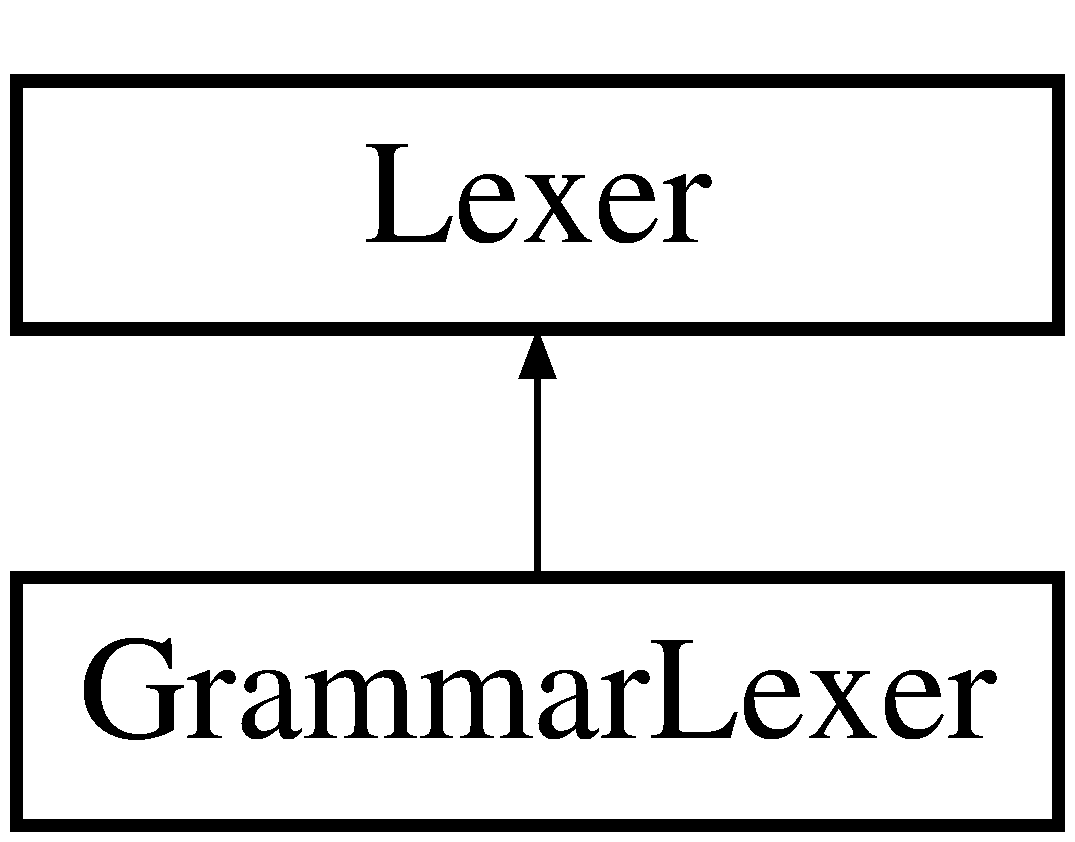
\includegraphics[height=2.000000cm]{classGrammarLexer}
\end{center}
\end{figure}
\subsection*{Открытые члены}
\begin{DoxyCompactItemize}
\item 
{\bf \-Grammar\-Lexer} (\-Q\-Text\-Stream \&strm)\label{classGrammarLexer_a755f5187a71b6b124a63cfb361dd4806}

\begin{DoxyCompactList}\small\item\em Создает лексический анализатор для указанного потока {\itshape strm\/}. \end{DoxyCompactList}\item 
virtual {\bf \-Token} {\bf next\-Token} ()
\begin{DoxyCompactList}\small\item\em Считывает новую лексему из потока преобразует в токен и возвращает этот токен \end{DoxyCompactList}\end{DoxyCompactItemize}
\subsection*{Статические открытые данные}
\begin{DoxyCompactItemize}
\item 
static const \-Q\-String {\bf deff\-Lexem} = \char`\"{}\-::=\char`\"{}\label{classGrammarLexer_a0012543850a39d9b9c511a0b67317dea}

\begin{DoxyCompactList}\small\item\em лексема, соединяющая левую и правую часть правила грамматики \end{DoxyCompactList}\item 
static const {\bf \-Surround\-Chars} {\bf surround\-Chars} = {\bf \-Surround\-Chars}('$<$', '$>$')\label{classGrammarLexer_ade9c6fa3eb41a1dfb71115eefc17ae27}

\begin{DoxyCompactList}\small\item\em символы, в которые заключается имя неТерминала \end{DoxyCompactList}\end{DoxyCompactItemize}


\subsection{Подробное описание}
Лексический анализатор для работы с описанием КС-\/грамматики 

Обрабатывает файлы и прочие текстовые потоки построчно. Выделяя в строке отдельные лексемы левую (с одним нетерминалом) и правую (с одним и более символов грамматики) часть правила, символ их разделяющий. Правая часть разбивается на лексемы, соответствующие терминальным, нетерминальным символам и символу \char`\"{}$|$\char`\"{}, разделяющему несколько продукций для единой левой части. 

\subsection{Методы}
\index{\-Grammar\-Lexer@{\-Grammar\-Lexer}!next\-Token@{next\-Token}}
\index{next\-Token@{next\-Token}!GrammarLexer@{\-Grammar\-Lexer}}
\subsubsection[{next\-Token}]{\setlength{\rightskip}{0pt plus 5cm}{\bf \-Token} {\bf \-Grammar\-Lexer\-::next\-Token} (
\begin{DoxyParamCaption}
{}
\end{DoxyParamCaption}
)\hspace{0.3cm}{\ttfamily  [virtual]}}\label{classGrammarLexer_a0ceeafa346f3ac54ee116fe5b50812fe}


Считывает новую лексему из потока преобразует в токен и возвращает этот токен 

Анализирует символы входного потока построчно. В каждой строке пытается найти последовательность {\bfseries \-Ns\-M}, где {\bfseries \-N} -\/ нетерминальный символ, окруженный символами из surround\-Chars (угловыми скобками в системе БНФ); {\bfseries s} -\/ символ определения порождения ({\itshape \char`\"{}\-::=\char`\"{}\/} в системе БНФ) {\bfseries \-M} -\/ множество терминальных, нетерминальных символов и символа \char`\"{}$|$\char`\"{}.

Если строка входного потока не начинается с пары {\bfseries \-Ns}, то возвращает токен ошибки ({\itshape alias\/} = {\ttfamily \char`\"{}error\char`\"{}}, {\itshape is\-System\-Token\/} = {\ttfamily true}.

Каждая строка преобразуется в очередь токенов, откуда и происходит считывание очередного токена до тех пор, пока очередь не опустеет, после чего считывается новая строка и формируется новая очередь.

\begin{DoxyReturn}{Возвращает}
сформированный токен. 
\end{DoxyReturn}


Замещает {\bf \-Lexer} \doxyref{}{стр.}{classLexer}.



Объявления и описания членов классов находятся в файлах\-:\begin{DoxyCompactItemize}
\item 
\-Grammar\-Lexer.\-h\item 
\-Grammar\-Lexer.\-cpp\end{DoxyCompactItemize}

\section{Класс \-Grammar\-Symbol}
\label{classGrammarSymbol}\index{\-Grammar\-Symbol@{\-Grammar\-Symbol}}


Описывает символ грамматики  




{\ttfamily \#include $<$\-Grammar\-Symbol.\-h$>$}

\subsection*{Открытые члены}
\begin{DoxyCompactItemize}
\item 
{\bf \-Grammar\-Symbol} ()\label{classGrammarSymbol_a08cda21b11486c614c407756eb15112d}

\begin{DoxyCompactList}\small\item\em Создает грамматический пустой символ \end{DoxyCompactList}\item 
{\bf \-Grammar\-Symbol} (const \-Q\-String \&{\bf alias}, const \-Q\-String \&{\bf description}=\-Q\-String())
\begin{DoxyCompactList}\small\item\em Создает грамматический символ с указаннами псевдонимом и описанием \end{DoxyCompactList}\item 
bool {\bf is\-Terminal} () const 
\begin{DoxyCompactList}\small\item\em Проверяет, является ли символ терминальным \end{DoxyCompactList}\end{DoxyCompactItemize}
\subsection*{Открытые атрибуты}
\begin{DoxyCompactItemize}
\item 
\-Q\-String {\bf alias}\label{classGrammarSymbol_a6a9f9d16afbb53c9c4ea010ede942b27}

\begin{DoxyCompactList}\small\item\em псевдоним грамматического символа \end{DoxyCompactList}\item 
\-Q\-String {\bf description}\label{classGrammarSymbol_ab434f25b9bcbffebe9bdd0dc75489cb4}

\begin{DoxyCompactList}\small\item\em описание грамматического символа \end{DoxyCompactList}\item 
\-Q\-List$<$ \-Symbols\-Sequence $>$ {\bf products}\label{classGrammarSymbol_a6a23b1626b2ac5f91c0578f279d37315}

\begin{DoxyCompactList}\small\item\em продукции грамматического символа \end{DoxyCompactList}\end{DoxyCompactItemize}


\subsection{Подробное описание}
Описывает символ грамматики 

\subsection{Конструктор(ы)}
\index{\-Grammar\-Symbol@{\-Grammar\-Symbol}!\-Grammar\-Symbol@{\-Grammar\-Symbol}}
\index{\-Grammar\-Symbol@{\-Grammar\-Symbol}!GrammarSymbol@{\-Grammar\-Symbol}}
\subsubsection[{\-Grammar\-Symbol}]{\setlength{\rightskip}{0pt plus 5cm}{\bf \-Grammar\-Symbol\-::\-Grammar\-Symbol} (
\begin{DoxyParamCaption}
\item[{const \-Q\-String \&}]{alias, }
\item[{const \-Q\-String \&}]{description = {\ttfamily \-Q\-String()}}
\end{DoxyParamCaption}
)\hspace{0.3cm}{\ttfamily  [explicit]}}\label{classGrammarSymbol_a927b675aa1189d5aee5c31ce4cf123a5}


Создает грамматический символ с указаннами псевдонимом и описанием 


\begin{DoxyParams}{Аргументы}
{\em alias} & псевдоним грамматического символа. \\
\hline
{\em description} & описание грамматического символа \\
\hline
\end{DoxyParams}


\subsection{Методы}
\index{\-Grammar\-Symbol@{\-Grammar\-Symbol}!is\-Terminal@{is\-Terminal}}
\index{is\-Terminal@{is\-Terminal}!GrammarSymbol@{\-Grammar\-Symbol}}
\subsubsection[{is\-Terminal}]{\setlength{\rightskip}{0pt plus 5cm}bool {\bf \-Grammar\-Symbol\-::is\-Terminal} (
\begin{DoxyParamCaption}
{}
\end{DoxyParamCaption}
) const}\label{classGrammarSymbol_a6373e59fb6b26eda93238f31ba19c1b0}


Проверяет, является ли символ терминальным 

\begin{DoxyReturn}{Возвращает}
{\ttfamily true}, если символ терминальный (не содержит продукций), иначе {\ttfamily false} 
\end{DoxyReturn}


Объявления и описания членов классов находятся в файлах\-:\begin{DoxyCompactItemize}
\item 
\-Grammar\-Symbol.\-h\item 
\-Grammar\-Symbol.\-cpp\end{DoxyCompactItemize}

\section{Класс \-Lexer}
\label{classLexer}\index{\-Lexer@{\-Lexer}}


Лексический анализатор  




{\ttfamily \#include $<$\-Lexer.\-h$>$}

Граф наследования\-:\-Lexer\-:\begin{figure}[H]
\begin{center}
\leavevmode
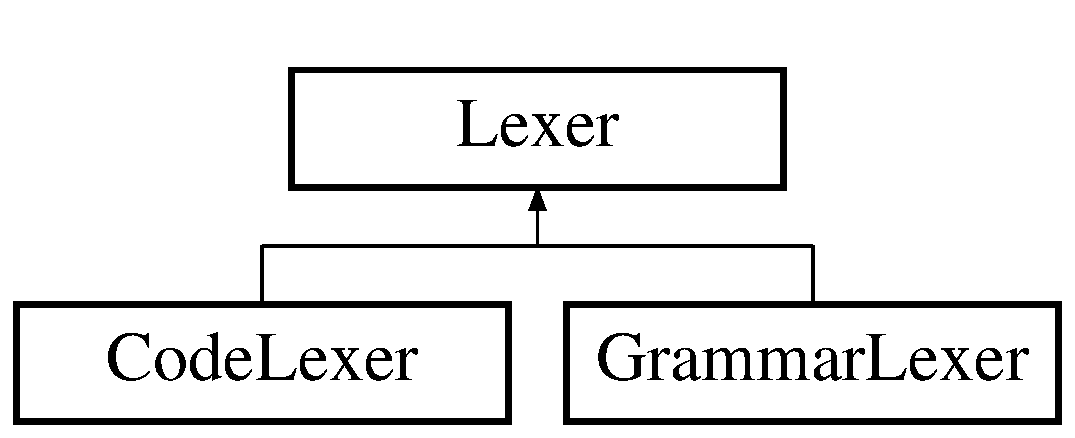
\includegraphics[height=2.000000cm]{classLexer}
\end{center}
\end{figure}
\subsection*{Открытые члены}
\begin{DoxyCompactItemize}
\item 
{\bf \-Lexer} (\-Q\-Text\-Stream \&strm)
\begin{DoxyCompactList}\small\item\em Создает лексический анализатор для обработки потока данных {\itshape strm\/}. \end{DoxyCompactList}\item 
{\bf \-Token} {\bf token} () const 
\begin{DoxyCompactList}\small\item\em Возвращает значение токена на основе последней считанной лексемы \end{DoxyCompactList}\item 
virtual {\bf \-Token} {\bfseries next\-Token} ()=0\label{classLexer_aefb597575e35cf11b0c207b4c279b26c}

\item 
const \-Q\-Text\-Stream \& {\bf stream} ()
\begin{DoxyCompactList}\small\item\em Возвращает ссылку на поток, с которым работает текущий экземпляр анализатора \end{DoxyCompactList}\end{DoxyCompactItemize}
\subsection*{Открытые атрибуты}
\begin{DoxyCompactItemize}
\item 
\-Q\-Set$<$ \-Q\-Char $>$ {\bf ignored\-Chars}\label{classLexer_aeeca22b6d3c00718ce6a6efdeecaf26c}

\begin{DoxyCompactList}\small\item\em Список игнорируемых символов \end{DoxyCompactList}\end{DoxyCompactItemize}
\subsection*{Защищенные данные}
\begin{DoxyCompactItemize}
\item 
\-Q\-Text\-Stream \& {\bf m\-\_\-strm}\label{classLexer_a5917fcd8a7a63ac287c52d92bae209ee}

\begin{DoxyCompactList}\small\item\em Поток для обработки \end{DoxyCompactList}\item 
{\bf \-Token} {\bf m\-\_\-token}\label{classLexer_a9d3564b81ee5782e1d17b91c32ea91c7}

\begin{DoxyCompactList}\small\item\em Текущий, уже считанный токен \end{DoxyCompactList}\end{DoxyCompactItemize}


\subsection{Подробное описание}
Лексический анализатор 

\subsection{Конструктор(ы)}
\index{\-Lexer@{\-Lexer}!\-Lexer@{\-Lexer}}
\index{\-Lexer@{\-Lexer}!Lexer@{\-Lexer}}
\subsubsection[{\-Lexer}]{\setlength{\rightskip}{0pt plus 5cm}{\bf \-Lexer\-::\-Lexer} (
\begin{DoxyParamCaption}
\item[{\-Q\-Text\-Stream \&}]{strm}
\end{DoxyParamCaption}
)\hspace{0.3cm}{\ttfamily  [explicit]}}\label{classLexer_a40eb253d60a387a79fd4fe5530cde54d}


Создает лексический анализатор для обработки потока данных {\itshape strm\/}. 


\begin{DoxyParams}{Аргументы}
{\em strm} & анализируемый поток \\
\hline
{\em white\-Spaces} & список игнорируемых символов \\
\hline
\end{DoxyParams}


\subsection{Методы}
\index{\-Lexer@{\-Lexer}!stream@{stream}}
\index{stream@{stream}!Lexer@{\-Lexer}}
\subsubsection[{stream}]{\setlength{\rightskip}{0pt plus 5cm}const \-Q\-Text\-Stream \& {\bf \-Lexer\-::stream} (
\begin{DoxyParamCaption}
{}
\end{DoxyParamCaption}
)}\label{classLexer_abf8dc6b2f227ccccba2f3285112698a9}


Возвращает ссылку на поток, с которым работает текущий экземпляр анализатора 

\begin{DoxyReturn}{Возвращает}
ссылка на обрабатываемый поток. 
\end{DoxyReturn}
\index{\-Lexer@{\-Lexer}!token@{token}}
\index{token@{token}!Lexer@{\-Lexer}}
\subsubsection[{token}]{\setlength{\rightskip}{0pt plus 5cm}{\bf \-Token} {\bf \-Lexer\-::token} (
\begin{DoxyParamCaption}
{}
\end{DoxyParamCaption}
) const}\label{classLexer_af0b127e33e42fe7a62b662f4eed71b22}


Возвращает значение токена на основе последней считанной лексемы 

\begin{DoxyReturn}{Возвращает}
последний считанный токен. 
\end{DoxyReturn}


Объявления и описания членов классов находятся в файлах\-:\begin{DoxyCompactItemize}
\item 
\-Lexer.\-h\item 
\-Lexer.\-cpp\end{DoxyCompactItemize}

\section{Структура \-Surround\-Chars}
\label{structSurroundChars}\index{\-Surround\-Chars@{\-Surround\-Chars}}


Описание символов, окружающих лексему  




{\ttfamily \#include $<$\-Grammar\-Lexer.\-h$>$}

\subsection*{Открытые члены}
\begin{DoxyCompactItemize}
\item 
{\bfseries \-Surround\-Chars} (char l, char r)\label{structSurroundChars_abc9876360349909ea958da1097635dc8}

\end{DoxyCompactItemize}
\subsection*{Открытые атрибуты}
\begin{DoxyCompactItemize}
\item 
char {\bf left}\label{structSurroundChars_a01aab228ec4e8d8d1d34215e9b817bb2}

\begin{DoxyCompactList}\small\item\em левый обрамляющий символ \end{DoxyCompactList}\item 
char {\bf right}\label{structSurroundChars_a18d7820ae790961c0e17b130571b4c38}

\begin{DoxyCompactList}\small\item\em правый обрамляющий символ \end{DoxyCompactList}\end{DoxyCompactItemize}


\subsection{Подробное описание}
Описание символов, окружающих лексему 

Объявления и описания членов структур находятся в файлах\-:\begin{DoxyCompactItemize}
\item 
\-Grammar\-Lexer.\-h\item 
\-Grammar\-Lexer.\-cpp\end{DoxyCompactItemize}

\section{Класс \-Table\-Driven\-Parser}
\label{classTableDrivenParser}\index{\-Table\-Driven\-Parser@{\-Table\-Driven\-Parser}}


Синтаксический нерекурсивный предиктивный анализатор \-L\-L(1)-\/грамматик  




{\ttfamily \#include $<$\-Table\-Driven\-Parser.\-h$>$}

\subsection*{Открытые члены}
\begin{DoxyCompactItemize}
\item 
{\bf \-Table\-Driven\-Parser} (\-Q\-Text\-Stream $\ast$error\-Out=0)
\begin{DoxyCompactList}\small\item\em Создает экземпляр синтаксического анализатора \end{DoxyCompactList}\item 
bool {\bf load\-Grammar} (const \-Q\-String \&file\-Path\-Name)
\begin{DoxyCompactList}\small\item\em Загружает описание \-L\-L(1) грамматики из файла для конфигурирования парсера \end{DoxyCompactList}\item 
void {\bf set\-Grammar} (const \-Q\-List$<$ {\bf \-Grammar\-Symbol} $>$ \&symbols)
\begin{DoxyCompactList}\small\item\em Создает внутреннее описание грамматики на основе переданого списка \end{DoxyCompactList}\item 
bool {\bf analyse} ({\bf \-Lexer} \&lexer, \-Q\-Dom\-Document \&result, bool is\-Parse\-Tree\-In\-Result=true)
\begin{DoxyCompactList}\small\item\em Анализирует входной поток {\itshape stream\/} на соответствие грамматике \end{DoxyCompactList}\end{DoxyCompactItemize}


\subsection{Подробное описание}
Синтаксический нерекурсивный предиктивный анализатор \-L\-L(1)-\/грамматик 

По указанному в виде файла описанию \-L\-L(1)-\/грамматики производит синтаксический разбор входного потока с использованнием указанного лексического анализатора.

Формирует дерево разбора в виде \-X\-M\-L-\/документа. 

\subsection{Конструктор(ы)}
\index{\-Table\-Driven\-Parser@{\-Table\-Driven\-Parser}!\-Table\-Driven\-Parser@{\-Table\-Driven\-Parser}}
\index{\-Table\-Driven\-Parser@{\-Table\-Driven\-Parser}!TableDrivenParser@{\-Table\-Driven\-Parser}}
\subsubsection[{\-Table\-Driven\-Parser}]{\setlength{\rightskip}{0pt plus 5cm}{\bf \-Table\-Driven\-Parser\-::\-Table\-Driven\-Parser} (
\begin{DoxyParamCaption}
\item[{\-Q\-Text\-Stream $\ast$}]{error\-Out = {\ttfamily 0}}
\end{DoxyParamCaption}
)}\label{classTableDrivenParser_a9567e9e506d8024a91125d5399ad23c5}


Создает экземпляр синтаксического анализатора 


\begin{DoxyParams}{Аргументы}
{\em error\-Out} & указатель на поток для вывода сообщений об ошибках анализа. \\
\hline
\end{DoxyParams}


\subsection{Методы}
\index{\-Table\-Driven\-Parser@{\-Table\-Driven\-Parser}!analyse@{analyse}}
\index{analyse@{analyse}!TableDrivenParser@{\-Table\-Driven\-Parser}}
\subsubsection[{analyse}]{\setlength{\rightskip}{0pt plus 5cm}bool {\bf \-Table\-Driven\-Parser\-::analyse} (
\begin{DoxyParamCaption}
\item[{{\bf \-Lexer} \&}]{lexer, }
\item[{\-Q\-Dom\-Document \&}]{result, }
\item[{bool}]{is\-Parse\-Tree\-In\-Result = {\ttfamily true}}
\end{DoxyParamCaption}
)}\label{classTableDrivenParser_ae6b177588fa192998df76d27ed290c34}


Анализирует входной поток {\itshape stream\/} на соответствие грамматике 

Производит анализ входного потока {\itshape stream\/} на соответствие грамматике, установленной для парсера с помощью \doxyref{load\-Grammar()}{стр.}{classTableDrivenParser_abbe14ed1158d653aaa1dcf0c256b7fda} или \doxyref{set\-Grammar()}{стр.}{classTableDrivenParser_a65fbc9f689d599a27b413b93cb8a109d}. Все ошибки, возникающие во время анализа выводятся либо в поток, заданный при создании объекта парсера, либо в stderr, если поток не был задан.

В случае успешного анализа функция возрващает {\ttfamily true} и заполняет переданную по ссылке конструкцию \-Q\-Dom\-Document деревом разбора (при {\itshape is\-Parse\-Tree\-In\-Result\/} = {\ttfamily true}, по умолчанию) или ситаксическим деревом (при {\itshape is\-Parse\-Tree\-In\-Result\/} = {\ttfamily false}).


\begin{DoxyParams}{Аргументы}
{\em lexer} & лексический анализатор, из которого будут получаться лексемы. \\
\hline
{\em result} & дерево разбора или синтаксическое дерево, в зависимости от {\itshape is\-Syntax\-Tree\-In\-Result\/} \\
\hline
{\em is\-Parse\-Tree\-In\-Result} & флаг, указывающий, что нужно строить дерево разбора, а не синтаксическое дерево \\
\hline
\end{DoxyParams}
\index{\-Table\-Driven\-Parser@{\-Table\-Driven\-Parser}!load\-Grammar@{load\-Grammar}}
\index{load\-Grammar@{load\-Grammar}!TableDrivenParser@{\-Table\-Driven\-Parser}}
\subsubsection[{load\-Grammar}]{\setlength{\rightskip}{0pt plus 5cm}bool {\bf \-Table\-Driven\-Parser\-::load\-Grammar} (
\begin{DoxyParamCaption}
\item[{const \-Q\-String \&}]{file\-Path\-Name}
\end{DoxyParamCaption}
)}\label{classTableDrivenParser_abbe14ed1158d653aaa1dcf0c256b7fda}


Загружает описание \-L\-L(1) грамматики из файла для конфигурирования парсера 

Файл должен содержать описание по системе БНФ. При описании разрешено использовать как латиницу, так и кириллицу. Для грамматики предопределены такие терминалы, как {\ttfamily \char`\"{}id\char`\"{}} для идентификаторов и {\ttfamily \char`\"{}num\char`\"{}} для вещественных и целых чисел, а так же {\ttfamily \char`\"{}empty\char`\"{}} для пустого символа.


\begin{DoxyParams}{Аргументы}
{\em file\-Path\-Name} & путь к файлу с описанием грамматики. \\
\hline
\end{DoxyParams}
\begin{DoxyReturn}{Возвращает}
{\ttfamily true}, если грамматика успешно загружена, иначе false. 
\end{DoxyReturn}
\index{\-Table\-Driven\-Parser@{\-Table\-Driven\-Parser}!set\-Grammar@{set\-Grammar}}
\index{set\-Grammar@{set\-Grammar}!TableDrivenParser@{\-Table\-Driven\-Parser}}
\subsubsection[{set\-Grammar}]{\setlength{\rightskip}{0pt plus 5cm}void {\bf \-Table\-Driven\-Parser\-::set\-Grammar} (
\begin{DoxyParamCaption}
\item[{const \-Q\-List$<$ {\bf \-Grammar\-Symbol} $>$ \&}]{symbols}
\end{DoxyParamCaption}
)}\label{classTableDrivenParser_a65fbc9f689d599a27b413b93cb8a109d}


Создает внутреннее описание грамматики на основе переданого списка 


\begin{DoxyParams}{Аргументы}
{\em symbols} & список символов грамматики и их продукций. \\
\hline
\end{DoxyParams}


Объявления и описания членов классов находятся в файлах\-:\begin{DoxyCompactItemize}
\item 
\-Table\-Driven\-Parser.\-h\item 
\-Table\-Driven\-Parser.\-cpp\end{DoxyCompactItemize}

\section{Структура \-Token}
\label{structToken}\index{\-Token@{\-Token}}


Токен полученный из лексемы входного потока  




{\ttfamily \#include $<$\-Lexer.\-h$>$}

\subsection*{Открытые члены}
\begin{DoxyCompactItemize}
\item 
{\bf \-Token} (\-Q\-String a=\-Q\-String(\char`\"{}empty\char`\"{}), \-Q\-Variant v=\-Q\-Variant(), int l=-\/1, int p=-\/1, bool is\-Sys=false)
\begin{DoxyCompactList}\small\item\em Создает токен с указанными параметрами \end{DoxyCompactList}\end{DoxyCompactItemize}
\subsection*{Открытые атрибуты}
\begin{DoxyCompactItemize}
\item 
\-Q\-String {\bf alias}\label{structToken_ab8e8a13e841bf54bf1dc802eb4557d3d}

\begin{DoxyCompactList}\small\item\em псевдоним для лексемы \end{DoxyCompactList}\item 
\-Q\-Variant {\bf value}\label{structToken_a3cb4743f3dd1dbc6bdfc84c415e9b37b}

\begin{DoxyCompactList}\small\item\em значение лексемы \end{DoxyCompactList}\item 
int {\bf line}\label{structToken_a4b96c2a31d7c374fd2bd1986794f80dd}

\begin{DoxyCompactList}\small\item\em номер строки входного потока, содержащей лексему \end{DoxyCompactList}\item 
int {\bf pos\-In\-Line}\label{structToken_aab7e25636c4dd8e2f873abd5b5435a17}

\begin{DoxyCompactList}\small\item\em позиция лексемы в строке входного потока \end{DoxyCompactList}\item 
bool {\bf is\-System\-Token}\label{structToken_ac77d1174920f71e83091e6d009b1f8a4}

\begin{DoxyCompactList}\small\item\em флаг системного токена (ошибки, конец потока) \end{DoxyCompactList}\end{DoxyCompactItemize}


\subsection{Подробное описание}
Токен полученный из лексемы входного потока 

\subsection{Конструктор(ы)}
\index{\-Token@{\-Token}!\-Token@{\-Token}}
\index{\-Token@{\-Token}!Token@{\-Token}}
\subsubsection[{\-Token}]{\setlength{\rightskip}{0pt plus 5cm}{\bf \-Token\-::\-Token} (
\begin{DoxyParamCaption}
\item[{\-Q\-String}]{a = {\ttfamily \-Q\-String(\char`\"{}empty\char`\"{})}, }
\item[{\-Q\-Variant}]{v = {\ttfamily \-Q\-Variant()}, }
\item[{int}]{l = {\ttfamily -\/1}, }
\item[{int}]{p = {\ttfamily -\/1}, }
\item[{bool}]{is\-Sys = {\ttfamily false}}
\end{DoxyParamCaption}
)}\label{structToken_adc69586500a7bf29d1f8d7108a88cbd3}


Создает токен с указанными параметрами 


\begin{DoxyParams}{Аргументы}
{\em a} & псевдоним токена. \\
\hline
{\em v} & значение токена. \\
\hline
{\em l} & номер строки в исходном потоке, содержащей токен. \\
\hline
{\em p} & позиция токена в строке {\itshape l\/} исходного потока. \\
\hline
{\em is\-Sys} & флаг того, является ли токен системным. \\
\hline
\end{DoxyParams}


Объявления и описания членов структур находятся в файлах\-:\begin{DoxyCompactItemize}
\item 
\-Lexer.\-h\item 
\-Lexer.\-cpp\end{DoxyCompactItemize}

\printindex
\end{document}
